% Drawing 161-6/01-4 -- folder 161-6, batch 01, archive page 16 (PDF page 17).
% Transcription: feuillet de carnet à spirale, en largeur, couvert d'une trentaine de croquis à l'encre et au crayon, mêlés de formules : fleurs à trois, quatre ou cinq pétales, dont l'une, en marge gauche, est légendée « corolle », « racine », « tige », « cœur », « pétale » ; une fleur à trois lobes à côté d'un disque noirci ; tétraèdres et pyramides, dont l'un, au crayon, avec un point intérieur relié aux sommets ; un losange à diagonales suivi d'un « $G$ » ; un hexagone découpé en six triangles, relié par un arc à un point près du « $G$ » et légendé « $\mathrm{O}(3)$ », « $\mathrm{SO}(3)$ » ; une suite de trois ovales emboîtés dont le plus intérieur porte « $u_1$ » et « $u_0$ » cerclé ; un carré inscrit dans un quadrilatère, reliés par les diagonales ; un graphe en forme de cube aplati, à sommets marqués de ronds, de croix et de points ; un cube dont trois faces sont fléchées vers un sommet ; un gros « 8 ».
% Kind: notebook leaf covered with sketches (flowers, polyhedra, nested ovals). Method 2 (schematic redraw from the facsimile). Status: partial.
% Notes: Whole leaf, about thirty small sketches in ink and pencil among formulas; only a selection is redrawn, each at its place on the leaf (1 unit = 1.8 mm): the flower of the left margin with its legends (heart, two petals, stem ending in a dot, the oval of the root; the words corolle, racine, tige, cœur, pétale written along the margin); the four-petalled flower with its stalk; the three-lobed flower (three closed lobes from one centre point) and the blackened disc beside it (hatched); the three nested ovals with u_1 and the circled u_0; the square inside a quadrilateral, corners joined; the hexagon cut into six triangles from its centre, the arc from it to the dot near « G », and « O(3) », « SO(3) »; the large pencil tetrahedron with an inner point joined to its three vertices; the heavy « 8 ». NOT redrawn: the small tetrahedra and pyramids of the top row and of the bottom row, the rhombus with diagonals, the leaf-shaped and lens-shaped outlines, the faint pencil circles, the two five-petalled flowers at the right, the two touching discs, the graph with marked vertices, the cube with arrows, the heavy quadrilateral figures at the top right and bottom right, the chain 4 -> 3 -> 2 -> 1 -> 0 and all the formulas (which the transcription gives). Disagreements with the transcription's note: the nested ovals are three (it says « une suite d'ovales emboîtés dont les deux plus intérieurs portent u_1 et u_0 »: both letters are inside the innermost oval); the graph it calls « sur six sommets » seems to have eight vertices (a square inside a square, corners joined), to be checked. Still differs: everything listed as not redrawn; the lobes and petals are smooth curves through a few read points. Redrawn 2026-11-10 (issue 128): to check again.
% Coordinates: 1 unit = 1.8 mm = 1/100 of the crop width (bbox in page fractions: [0.09, 0.065, 1.0, 0.49]).
% Redrawn by Claude (claude-fable-5-2), issue #128, 2026-11-10; not checked by a human; not compiled (no TeX in the session).
% Rights: reproduces part of the work -- behind RENDER_TRANSCRIPTS, never published by itself.
\documentclass[tikz,border=3pt]{standalone}
\usepackage{amsmath,amssymb}
\usetikzlibrary{patterns,arrows.meta}
\tikzset{pencil/.style={black!45}, struck/.style={black!35}, mpt/.style={circle,draw,inner sep=1.3pt}, pt/.style={circle,fill,inner sep=0.9pt}, opt/.style={circle,draw,fill=white,inner sep=1.1pt}}
\begin{document}
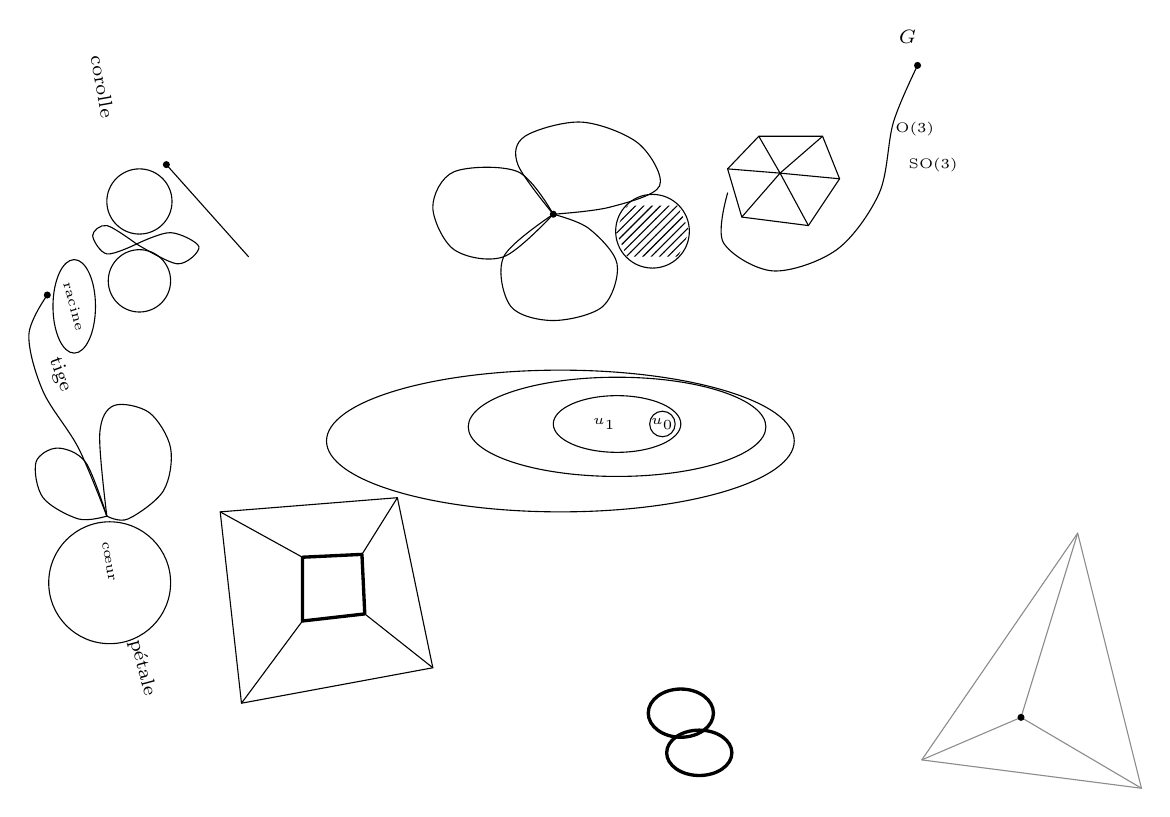
\begin{tikzpicture}[x=1.8mm,y=1.8mm,line cap=round,line join=round,font=\scriptsize]
\draw (10.7,-49.5) circle[radius=4.3];
\draw plot[smooth, tension=0.55] coordinates {(10.5,-44.8) (8.5,-45) (6,-43.5) (5.5,-41) (7,-40) (9,-41) (10.5,-44.8)};
\draw plot[smooth, tension=0.55] coordinates {(10.5,-44.8) (10,-39) (11,-37) (13.5,-37.5) (15,-40) (14.5,-43) (12,-45) (10.5,-44.8)};
\draw plot[smooth, tension=0.55] coordinates {(10.5,-44.8) (8.5,-40) (6,-36) (5,-32) (6.3,-29.2)};
\node[pt] at (6.3,-29.2) {};
\draw (8.2,-30) ellipse[x radius=1.5, y radius=3.3];
\node[inner sep=1pt,rotate=-80] at (10.2,-14.5) {\scriptsize corolle};
\node[inner sep=1pt,rotate=-75] at (8.2,-30) {\tiny racine};
\node[inner sep=1pt,rotate=-70] at (7.2,-34.8) {\scriptsize tige};
\node[inner sep=1pt,rotate=-80] at (10.6,-48) {\tiny cœur};
\node[inner sep=1pt,rotate=-75] at (13,-55.5) {\scriptsize pétale};
\draw (12.8,-22.6) circle[radius=2.3];
\draw (12.8,-28.2) circle[radius=2.2];
\draw plot[smooth, tension=0.55] coordinates {(12.6,-25.6) (10.5,-24.3) (9.5,-25) (10.5,-26.3) (12.6,-25.6)};
\draw plot[smooth, tension=0.55] coordinates {(12.6,-25.6) (15,-24.8) (17,-25.8) (15.5,-27) (12.6,-25.6)};
\draw (14.7,-20) -- (20.5,-26.5);
\node[pt] at (14.7,-20) {};
\draw plot[smooth, tension=0.55] coordinates {(42,-23.5) (39.5,-20) (40,-18) (44,-17) (48,-18.5) (49.5,-21.5) (46,-23) (42,-23.5)};
\draw plot[smooth, tension=0.55] coordinates {(42,-23.5) (39.5,-20.5) (35,-20.5) (33.5,-23) (35,-26) (38.5,-26.5) (42,-23.5)};
\draw plot[smooth, tension=0.55] coordinates {(42,-23.5) (38.5,-26.5) (39,-30) (42,-31) (45.5,-30) (46.5,-27) (44.5,-24.5) (42,-23.5)};
\node[pt] at (42,-23.5) {};
\draw (49,-24.7) circle[radius=2.6];
\fill[pattern=north east lines] (47.2,-22.9) -- (50.8,-22.9) -- (51.6,-24.7) -- (50.8,-26.5) -- (47.2,-26.5) -- (46.4,-24.7) -- cycle;
\draw (46.5,-38.3) ellipse[x radius=4.5, y radius=2];
\draw (46.5,-38.5) ellipse[x radius=10.5, y radius=3.5];
\draw (42.5,-39.5) ellipse[x radius=16.5, y radius=5];
\node[inner sep=1pt] at (45.6,-38.3) {\tiny $u_1$};
\node[inner sep=1pt] at (49.7,-38.3) {\tiny $u_0$};
\draw (49.7,-38.3) circle[radius=0.9];
\draw (18.5,-44.5) -- (31,-43.5) -- (33.5,-55.5) -- (20,-58) -- cycle;
\draw[very thick] (24.3,-47.7) -- (28.5,-47.5) -- (28.7,-51.7) -- (24.3,-52.2) -- cycle;
\draw (18.5,-44.5) -- (24.3,-47.7);
\draw (31,-43.5) -- (28.5,-47.5);
\draw (33.5,-55.5) -- (28.7,-51.7);
\draw (20,-58) -- (24.3,-52.2);
\draw (56.5,-18) -- (61,-18) -- (62.2,-21) -- (60,-24.3) -- (55.3,-23.7) -- (54.3,-20.3) -- cycle;
\draw (58,-20.6) -- (56.5,-18);
\draw (58,-20.6) -- (61,-18);
\draw (58,-20.6) -- (62.2,-21);
\draw (58,-20.6) -- (60,-24.3);
\draw (58,-20.6) -- (55.3,-23.7);
\draw (58,-20.6) -- (54.3,-20.3);
\draw plot[smooth, tension=0.55] coordinates {(67.7,-13) (66,-17) (65,-22) (62,-26) (57.5,-27.5) (54,-25.5) (54.3,-22)};
\node[pt] at (67.7,-13) {};
\node[inner sep=1pt] at (67.5,-17.5) {\tiny $\mathrm{O}(3)$};
\node[inner sep=1pt] at (68.8,-20) {\tiny $\mathrm{SO}(3)$};
\node[inner sep=1pt] at (67,-11) {\scriptsize $G$};
\draw[pencil] (79,-46) -- (68,-62) -- (83.5,-64) -- cycle;
\draw[pencil] (75,-59) -- (79,-46);
\draw[pencil] (75,-59) -- (68,-62);
\draw[pencil] (75,-59) -- (83.5,-64);
\node[pt] at (75,-59) {};
\draw[very thick] (51,-58.7) ellipse[x radius=2.3, y radius=1.7];
\draw[very thick] (52.3,-61.5) ellipse[x radius=2.3, y radius=1.6];
\end{tikzpicture}
\end{document}
